%==========================
%    PACKAGES AND THEMES
%==========================

\documentclass[aspectratio=169,xcolor=dvipsnames]{beamer}
%\usetheme{SimpleDarkBlue}
\usepackage{novabeamer}  % Use the custom theme
\usepackage{hyperref}
\usepackage{graphicx} % Allows including images
\usepackage{booktabs} % Allows the use of \toprule, \midrule and \bottomrule in tables
\usepackage{fontawesome5}


%==========================
%    TITLE PAGE
%==========================

\title{Catchy Title}
\subtitle{Subtitle}

\author{Riccardo Martelli}
\institute
{Institutions}
\date{\today} 

%==========================
%    PRESENTATION SLIDES
%==========================

\begin{document}

\begin{frame}
    \titlepage
\end{frame}

\begin{frame}{Overview}
    \tableofcontents
\end{frame}

%==========================
\section{GitHub Section}
%==========================

\begin{frame}{GitHub Hyperref link}
\centering
    \Huge Published on GitHub\\
    \href{https://github.com/Riccardo-Martelli/Riccardo-Beamer-Theme}{\faGithub GitHub link}
\end{frame}

%==========================

\begin{frame}{Formulas and Highlighted Text}

    In this slide, some important text will be \alert{highlighted}.

    \begin{block}{Text block describing the context}
        Text introducing a formula...
    \end{block}

    \begin{alertblock}{Formula}
        Sample text in red box...
        \[ds^2 = g_{\mu\nu}\, dx^\mu dx^\nu\,,\]
    \end{alertblock}

    \begin{examples}
        Sample text in green box describing Kerr Metric....
        \[ds^2 = \dots\]
    \end{examples}

    
\end{frame}

%==========================

\section{Section}

\begin{frame}{Multiple Columns}
    \begin{columns}[c] % The "c" option specifies centered vertical alignment while the "t" option is used for top vertical alignment

        \column{.45\textwidth} % Left column and width
        \textbf{List Title}
        \begin{enumerate}
            \item Statement
            \pause
            \item Explanation
            \pause
            \item Example $\quad\Longrightarrow$
        \end{enumerate}

        \column{.45\textwidth} % Right column and width
        \textbf{Example}\\
        Lorem ipsum dolor sit amet, consectetur adipiscing elit. Integer lectus nisl, ultricies in feugiat rutrum, porttitor sit amet augue. Aliquam ut tortor mauris. Sed volutpat ante purus, quis accumsan dolor.

    \end{columns}
\end{frame}

%==========================
\section{Another Section}
%==========================

\begin{frame}{Table}
    \begin{table}
        \begin{tabular}{c c c}
            \toprule
            \textbf{Portfolio} & \textbf{Risk Parity} & \textbf{Partial Sharpe Ratio} \\
            \midrule
            Asset 1         & 0.0003262           & 0.562               \\
            Asset 2         & 0.0015681           & 0.910               \\
            Asset 3         & 0.0009271           & 0.296               \\
            \bottomrule
        \end{tabular}
        \caption{Table caption}
    \end{table}
\end{frame}

%==========================

\begin{frame}{Theorem}
    \begin{theorem}[Lagrange's Mean Value Theorem ]
The \textbf{Mean Value Theorem (MVT)} states that if a function \( f \) is continuous on a closed interval \( [a,b] \) and differentiable on the open interval \( (a,b) \), then there exists at least one point \( c \) in \( (a,b) \) such that:

\[
f'(c) = \frac{f(b) - f(a)}{b - a}
\]
    \end{theorem}
\end{frame}

%==========================

\begin{frame}{Figure}
    Example of the usage of \textit{figure}. The image file is located in the same directory as the .tex file.
    \begin{figure}
    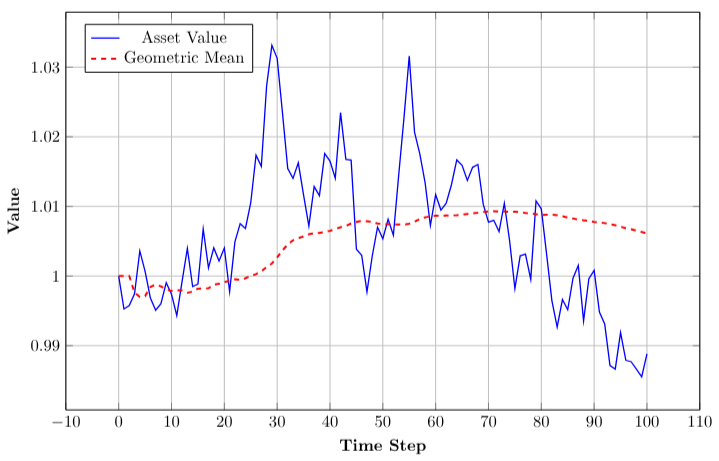
\includegraphics[width=0.6\linewidth]{examples/novabeamer-example-image.png.png}
    \end{figure}
\end{frame}

%==========================

\begin{frame}[fragile] % Need to use the fragile option when verbatim is used in the slide
    \frametitle{Citation}
    An example of the \verb|\cite| command to cite within the presentation:\\~

    Here is what a citation looks like \cite{p1}.
\end{frame}

%==========================

\begin{frame}{Bibliography/References}
    \nocite{*}
    \footnotesize
    \bibliography{examples/novabeamer-ref}
    \bibliographystyle{apalike}
\end{frame}

%==========================

\begin{frame}
\centering
    \vspace*{\fill}
    \fontsize{50}{60}{\centerline{\textbf{The End}}}
\end{frame}

%==========================

\end{document}